\documentclass[a0paper,landscape]{baposter}

\usepackage{relsize}		% For \smaller
\usepackage{epstopdf}	% Included EPS files automatically converted to PDF to include with pdflatex
\usepackage{float}
\usepackage{wrapfig}
\usepackage{minted}
\usepackage[none]{hyphenat}
\usepackage[sfdefault]{roboto}  %% Option 'sfdefault' only if the base font of the document is to be sans serif
\usepackage[T1]{fontenc}
\usepackage{multicol}

\usepackage{enumitem}
\setlist[itemize]{leftmargin=*,itemsep=0.5pt}

\renewcommand{\figurename}{\color{blue}Figure\color{black}}

%%% Global Settings %%%%%%%%%%%%%%%%%%%%%%%%%%%%%%%%%%%%%%%%%%%%%%%%%%%%%%%%%%%

\graphicspath{{pix/}}	% Root directory of the pictures 
\tracingstats=2			% Enabled LaTeX logging with conditionals

%%% Color Definitions %%%%%%%%%%%%%%%%%%%%%%%%%%%%%%%%%%%%%%%%%%%%%%%%%%%%%%%%%

\definecolor{bordercol}{RGB}{68,68,68}
\definecolor{headercol1}{RGB}{254,210,11}
\definecolor{headercol2}{RGB}{242,121,0}
\definecolor{headerfontcol}{RGB}{0,0,0}
\definecolor{boxcolor}{RGB}{255,255,230}

%%%%%%%%%%%%%%%%%%%%%%%%%%%%%%%%%%%%%%%%%%%%%%%%%%%%%%%%%%%%%%%%%%%%%%%%%%%%%%%%
%%% Utility functions %%%%%%%%%%%%%%%%%%%%%%%%%%%%%%%%%%%%%%%%%%%%%%%%%%%%%%%%%%

%%% Save space in lists. Use this after the opening of the list %%%%%%%%%%%%%%%%
\newcommand{\compresslist}{
	\setlength{\itemsep}{1pt}
	\setlength{\parskip}{0pt}
	\setlength{\parsep}{0pt}
}

%%%%%%%%%%%%%%%%%%%%%%%%%%%%%%%%%%%%%%%%%%%%%%%%%%%%%%%%%%%%%%%%%%%%%%%%%%%%%%%
%%% Document Start %%%%%%%%%%%%%%%%%%%%%%%%%%%%%%%%%%%%%%%%%%%%%%%%%%%%%%%%%%%%
%%%%%%%%%%%%%%%%%%%%%%%%%%%%%%%%%%%%%%%%%%%%%%%%%%%%%%%%%%%%%%%%%%%%%%%%%%%%%%%

\begin{document}
\typeout{Poster rendering started}

%%% Setting Background Image %%%%%%%%%%%%%%%%%%%%%%%%%%%%%%%%%%%%%%%%%%%%%%%%%%
\background{}

%%% General Poster Settings %%%%%%%%%%%%%%%%%%%%%%%%%%%%%%%%%%%%%%%%%%%%%%%%%%%
%%%%%% Eye Catcher, Title, Authors and University Images %%%%%%%%%%%%%%%%%%%%%%
\begin{poster}{
	grid=false,
	% Option is left on true though the eyecatcher is not used. The reason is
	% that we have a bit nicer looking title and author formatting in the headercol
	% this way
	eyecatcher=true, 
	borderColor=blue,
	headerColorOne=blue,
	headerColorTwo=blue,
	headerFontColor=white,
	% Only simple background color used, no shading, so boxColorTwo isn't necessary
	boxColorOne=white,
	headershape=rectangle,
	headerborder=open,
	headerfont=\Large\sf\bf,
	textborder=rectangle,
	background=none,
	headerborder=open,
    boxshade=plain,
    columns=4
}
%%% Title %%%%%%%%%%%%%%%%%%%%%%%%%%%%%%%%%%%%%%%%%%%%%%%%%%%%%%%%%%%%%%%%%%%%%
{
\includegraphics[height=4em]{images/diamondlogo}} 
{\bf \color{blue} Syringe Pump for Electrochemical Cell \vspace{0.5em}} % Poster title
{\textbf{Dolica Akello-Egwel}, Gary Yendell \hspace{12pt} 2018 Cohort / Mantid Team} % Author names and institution
{
\includegraphics[height=4em]{images/stfclogo}} 
%%%% Column 1 %%%%%%%%%%%%%%%%%%%%%%%%%%%%%%%%%%%%%%%%%%%%%%%%%%%%%%%%%%%%%%%%%%
%----------------------------------------------------------------------------------------
%	INTRODUCTION
%----------------------------------------------------------------------------------------
\begin{posterbox}[name=introduction,column=0]{Introduction}
The existing streamDevice-based EPICS driver for the Hamilton Microlab 500/600 Syringe Pump was not
especially suited to sending "complex" commands that contain two or more instructions.
The driver also lacked the ability to reliably send simultaneous commands to both syringes, and to
cycle sets of simultaneous commands indefinetly. The aim of this project was to create a user-friendly
and extensible Python API that addresses these issues and enables users to easily create continuous flows 
through an electrochemical cell.
\begin{figure}[H]
\begin{center}
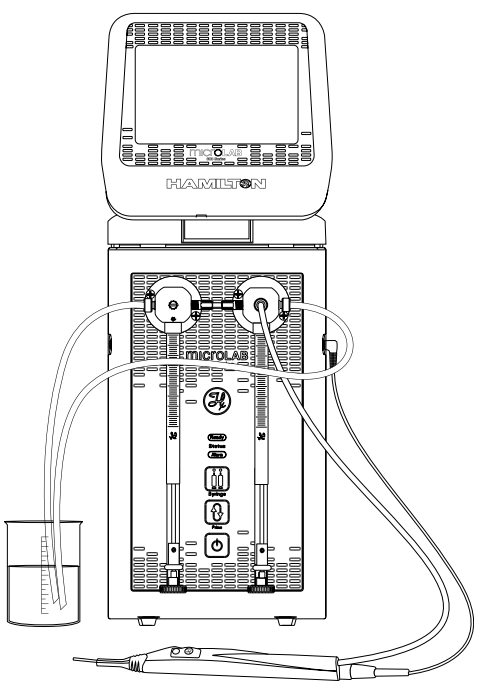
\includegraphics[width=100pt]{images/syringediagram}
\caption{Diagram of the syringe pump}
\end{center}
\end{figure}
\end{posterbox}
%----------------------------------------------------------------------------------------
%	REMOTE WORK
%----------------------------------------------------------------------------------------
\begin{posterbox}[column=0,headerfont={},headershape=rounded,boxheaderheight=0em,boxColorOne=white,borderColor=white,below=introduction]{rounded}
\begin{figure}[H]
\begin{center}
\vspace{-1em}
\frame{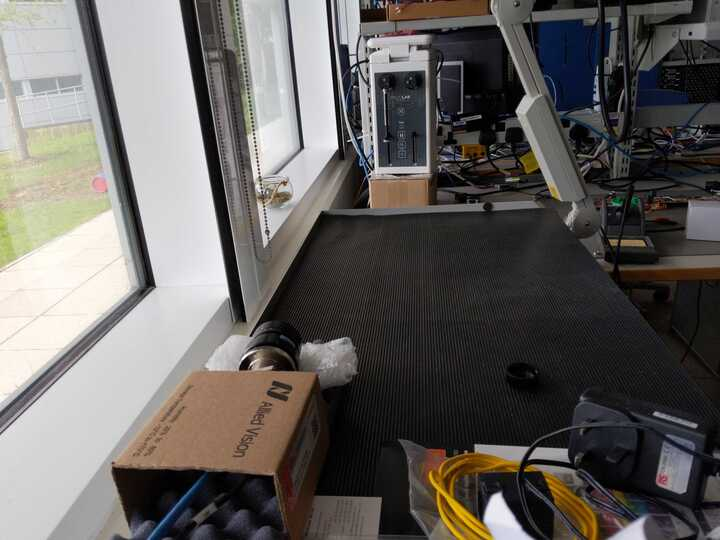
\includegraphics[width=\textwidth]{images/camerasetup}}
\caption{Remote working setup}
\end{center}
\end{figure}
\end{posterbox}
%%%% Column 2 %%%%%%%%%%%%%%%%%%%%%%%%%%%%%%%%%%%%%%%%%%%%%%%%%%%%%%%%%%%%%%%%%%
%----------------------------------------------------------------------------------------
%	OBJECTIVES
%----------------------------------------------------------------------------------------
\begin{posterbox}[name=objectives,column=1,row=0,span=2]{Objectives}
 \begin{itemize}
    \item Make a Python library for controlling the Hamilton Microlab Syringe Pump
    \item Allow the library to be controlled with a command-line interface 
    \item Add a cycling ability to allow the manipulation of continuous flows
    \item Allow the syringe paramters to be controlled via EPICS 
    \item Create a graphical interface using EDM screens
\end{itemize}
\end{posterbox}
%----------------------------------------------------------------------------------------
%	IMPLEMENTATION
%----------------------------------------------------------------------------------------
\begin{posterbox}[name=implementation,column=1,span=2,below=objectives]{Implementation}
\begin{minted}{python}
def _cycle_commands(
    self, commands: List[Command], address: str,
):
    while not self._stop_requested:
        for command in commands:
            self.send_command(command, address)
            while (
                self._comms.send_receive(address + INSTRUMENT_DONE)[1]
                != Y_INFO_RESPONSE
            ):
                if self._stop_requested:
                    self._reset_cycle(address)
                    return
                sleep(0.1)
    self._reset_cycle(address)
\end{minted}
\end{posterbox}
%----------------------------------------------------------------------------------------
%	CYCLING + CLI
%----------------------------------------------------------------------------------------
\begin{posterbox}[name=cycling,column=1,span=2,below=implementation]{Cycling and Command Line Interface}
    \begin{minted}{python}
        
    In [1]: speed = 20

    In [2]: empty_right_subcommands = [
    ...:     SyringeDispense(syringe=Side.RIGHT, value=MAX_SYRINGE_MOVE, speed=speed),
    ...:     SyringePickup(syringe=Side.LEFT, value=MAX_SYRINGE_MOVE, speed=speed),
    ...: ]

    In [3]: empty_left_subcommands = [
    ...:     SyringeDispense(syringe=Side.LEFT, value=MAX_SYRINGE_MOVE, speed=speed),
    ...:     SyringePickup(syringe=Side.RIGHT, value=MAX_SYRINGE_MOVE, speed=speed),
    ...: ]

    In [4]: microlab.cycle_commands(
    ...:     [Command(empty_right_subcommands), Command(empty_left_subcommands)]
    ...: )
    \end{minted}
\end{posterbox}
%%%% Column 3 %%%%%%%%%%%%%%%%%%%%%%%%%%%%%%%%%%%%%%%%%%%%%%%%%%%%%%%%%%%%%%%%%%
%----------------------------------------------------------------------------------------
%	EDM IMAGE
%----------------------------------------------------------------------------------------
\begin{posterbox}[name=edmimage,column=3,headerfont={},headershape=rounded,boxheaderheight=0em,boxColorOne=white,borderColor=white]{rounded}
\begin{figure}[H]
\begin{center}
\frame{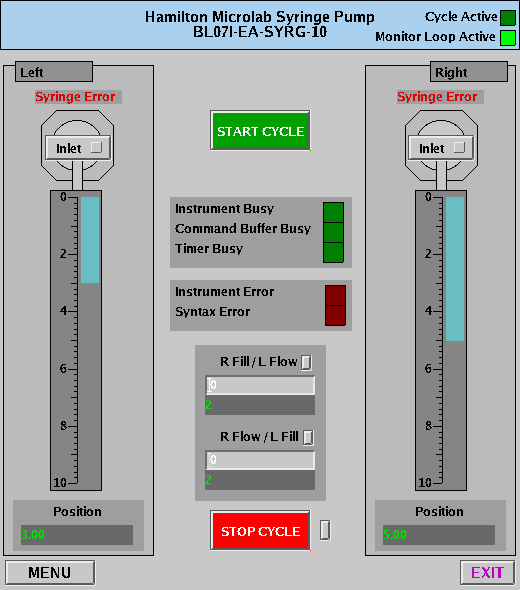
\includegraphics[width=\textwidth]{images/cycleedm}}
\caption{EDM screen for controlling command cycling}
\end{center}
\end{figure}
\end{posterbox}
%----------------------------------------------------------------------------------------
%	EDM SCREENS
%----------------------------------------------------------------------------------------
\begin{posterbox}[name=edmscreenexp,column=3,below=edmimage]{EDM Screens}
\end{posterbox}
%----------------------------------------------------------------------------------------
%	FUTURE WORK
%----------------------------------------------------------------------------------------
\begin{posterbox}[name=futurework,column=3,above=bottom]{Future Work}
 \begin{itemize}
    \item Write a simulation for the syringe pump 
    \item Add a cleaning command to the library with a corresponding button on the EDM screen 
    \item Enable syringe volumes to be changed on the fly 
    \item Accomodate daisy-chaining multiple syringe pumps 
\end{itemize}
\end{posterbox}

\end{poster}
\end{document}
